\documentclass[12pt]{article}
\usepackage{geometry}
\usepackage{graphicx}
\usepackage{float}
\usepackage{listings}

\lstset{frame=tb,
  language=bash,
  aboveskip=3mm,
  belowskip=3mm,
  showstringspaces=false,
  columns=flexible,
  basicstyle={\small\ttfamily},
  numbers=none,
  numberstyle=\tiny\color{gray},
  keywordstyle=\color{blue},
  commentstyle=\color{dkgreen},
  stringstyle=\color{mauve},
  breaklines=true,
  breakatwhitespace=true,
  tabsize=3
}
\begin{document}

\begin{flushright}
140024255\\
CS3105\\
Practical 2, Neural Nets
\end{flushright}

This practical tests the uses of a neural net for learning a classification problem as well as training a neural net to be a finite state machine.

\section{20 Questions}
\paragraph*{Pre-Processing and Input}
The system reads in input from two files: a concept to output pairing file and a concept to question-answer sequence file, both CSVs. This allows a concept to map to its question answers as well as the concept's binary output to map to its name (string). The input for the concept pairing is simple: two entries per line with the ideal output first (in decimal) and then the name. The input for the question answer mapping begins with one line that lists the questions (and an unused first entry). The rest of the lines map to the concept's ideal output in the net and its question answers. 
The program will then train on the input until the net correctly matches the question, answer, and concept mapping. It then goes into the play mode where it tries to guess the concept (all animals for this program) that the user is thinking about given user's answers to the question inputs. If the concept given by the net was incorrect, the net will try to learn a user's concept if the user tells it that the originally given concept was incorrect. However, if the input of one concept is the same as another (i.e., questions are answered the same for two concepts), the program's behavior is unexpected.

\paragraph*{Hidden Layering}
The fixed system starts off with 4 hidden units, as it allows the system to separate from the 16 beginning concepts. This is the threshold that allows for the separation of the starting concepts; 3 or lower hidden units will keep training and not reach the desired LMS error rate. For the learning system, hidden units are added when the number of epochs reaches 200,000. This is because, given my learning rate and momentum, the epochs will occasionally reach into the 100,000-plus range while also eventually reaching the desired error level. However, when the epoch number reaches the 200 or 300,000 range, it begins to plateau and will not train to the desired level. These values are taken from 5 new concepts onward since the error rate usually does not take that long to plateau when just adding one or two. The program then breaks out of training to add a hidden unit (if there is still classification error) and begins retraining.

\paragraph*{Output and Post-Processing}
The program will output the best concept matching the user's answers to the questions. Even if the input is incorrect, the program will output what it thinks is the correct answer (usually wrong). However, if the input completely matches an existing concept's input, the output is uncertain and training may not even complete.

\paragraph*{Training}
Training is done in both systems using backpropagation. Training for the fixed system has been tweaked for the best training time possible and correct results. It then takes the question-answer mapping for each concept as training input and the corresponding concept as output. For the fixed system, the learning rate is set to .06 and the momentum is .1. The program then trains until the error is less than or equal to .001 (the net is accurate in all tests at this level).
Training to learn a new concept builds off the concept, question, and answer inputs. Training to learn the new concept involves adding the new concept and its answers to the existing tables. Training grabs the number of hidden units from the last network, so that it doesn't waste training cycles adding more hidden units when it already knows at least how many it needs. The training process is similar to that of the fixed system in that it uses the Q&A mapping for the concepts as input and the concept value as ideal output. The training then aims for an LMS error of .001. If this level is reached, classification errors are eliminated. However, if the training is stuck around a certain error rate without decreasing, the epoch time out value will stop the training. After the training, if there are no classification errors, the system will resume playing with the new net. However, if there is still classification error, then hidden units are added and the entire process repeats.

\paragraph*{Choosing a Question}
Choosing a question has not been implemented due to time constraints. A good way of choosing the best question would be to keep track of concepts that have not been ruled out (at the beginning, all of them are in contention, which is why the first question should be one that best evenly divides the concepts). Given the list of concepts that have not been ruled out, one should then pick the next question that evenly divides the concepts. Since the system doesn't know the answer to the question beforehand, it can be wasteful to find the question that rules out the most concepts as the opposite answer would only rule out one. 

\paragraph*{When to Guess}
When to guess has not been implemented due to time constraints. The naive method to guess would be for when one of the concepts is separated from the rest. However, one method of guessing using more of a heuristic approach rather than a certain one (sacrificing some accuracy for faster guessing) would be to look at the raw outputs and accounting for how close they are to the extremes of 0 and 1. If enough of the outputs are close, the system should be able to guess with very good accuracy.

\paragraph*{Answers to Questions}
My system is limited by the questions in the input table. It can scale to, at most, twice the original size. If I were to ask the user for a question to distinguish the concept from the other similar ones, as well as the answer to this question for the other concepts, this would make the system very scalable since the system would now be able to dynamically grow very quickly. The one limit on this scalability, of course, is the user's ability to provide such questions and answers.
The system is very fault tolerant in accepting inputs. It is less so when training new concepts as it is unable to train concepts with question answer mappings that already exist. Finally, in terms of output, the system is not very fault tolerant. This is because the concepts are so closely grouped together that it is hard to distinguish between them when one answer is wrong.
%What are the similarities and differences between the way your system generalizes and standard neural generalization
 Since my system is a neural net trying to generalize a characterization problem, it has a lot in common with standard neural generalization problems. Like standard generalization problems, there are also many different possible generalizations. So, the system tries to fit the true relationship. Data for my system, like a standard neural generalization, can contain noise like a user incorrectly answering a question. Underfitting and overfitting are both concerns in this system and standard generalization ones. A significant difference between the my system and a standard neural generalization problem would be the pre-structured data. Whereas a neural net would normally use a sample of the possible data (usually a very small one, too since there may be infinitely many data sets). My static system does know the exact relationship between the input and output. There are only so many inputs and then they can only map to so many outputs, unlike neural nets that deal with much more spread out data. 

\begin{figure}
\centering
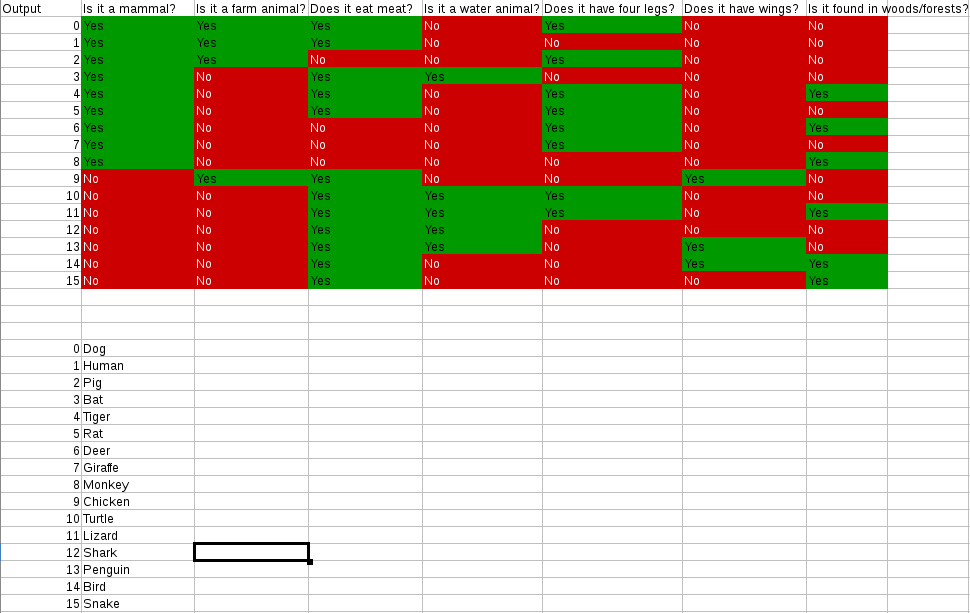
\includegraphics[width=350]{mappingtable.png}
\caption{Table for question set-answer and concept-output pairings.}
\end{figure}

\paragraph*{I/O}
The input tables also come with a spreadsheet to better view them. The spreadsheet (Figure 1) just shows the two tables in a more readable manner. As seen in the figure, each concept output (to the left, numbered from 0 to 15) is mapped to a set of answers to the questions on the top row. For example, The concept output is then mapped to the concept's name in another CSV file (shown below the question-answer mapping in the spreadsheet image).

Figures 2 and 3 show the net giving the incorrect concept to the user, the user giving the correct concept to the net, and then the net giving the correct concept to the user after learning the new concept.

\begin{figure}
\centering
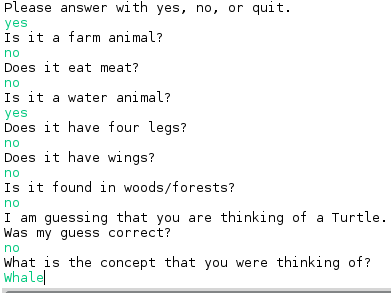
\includegraphics[width=350]{incorrect_input.png}
\caption{The user gives an unknown question-answer pattern to the net. The net tries to guess but is wrong, so the user supplies the concept.}
\end{figure}

\begin{figure}
\centering
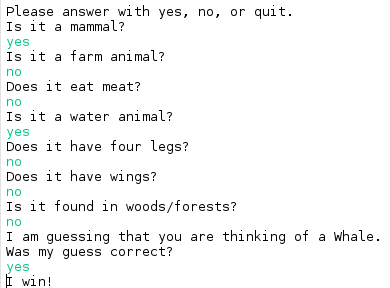
\includegraphics[width=350]{learnedconcept.png}
\caption{The net learns the new concept and gives the correct concept with the same question-answer pattern.}
\end{figure}

\paragraph*{Extension}
%Evaluate how well your system keeps the number of hidden units under control. Improve your system to keep the number of hidden units under better control.
Because my system takes a conservative approach to adding hidden units (given my parameters, I set the epoch time out to the time when the error rate stops decreasing and begins to plateau), it is already quite efficient. This method makes sure that the system needs to add hidden units, rather than because the learning rate and momentum were poorly chosen. Originally, the error weight was set a bit higher and the epoch time out lower. This didn't allow the program to train until it needed a new unit. This is because it stopped too quickly and just added another hidden unit to deal with a classification error. In addition to this, I also adjusted the hidden units of the fixed system to the lowest possible value with the system still performing correctly. While this sacrifices training speed, some of this is offset by setting better learning and momentum parameters.

\paragraph*{Documentation}
The 20Q program is located in the twentyq directory. The jar for it is located in the jar directory.
Run the jar with
\begin{verbatim}
java -jar 20QLearning.jar
\end{verbatim}
Compile the code by running
\begin{verbatim}
make
\end{verbatim}
Run the code with
\begin{verbatim}
java -cp .:encog.jar FileTrainer
\end{verbatim}

\begin{figure}
\centering
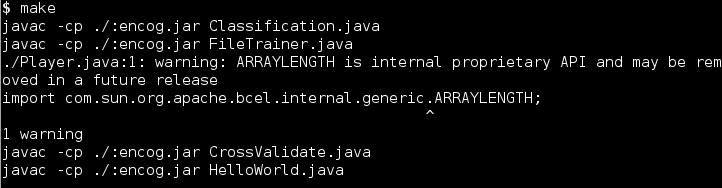
\includegraphics[width=350]{compile20q.png}
\caption{A screenshot of 20Q compiling.}
\end{figure}
\begin{figure}
\centering

\includegraphics[width=350]{run20q.png}
\caption{A screenshot of 20Q running.}
\end{figure}


\section{Self Programming}
For this part of the practical, I moved from trying a simple oscillating function given the same input. After that, I tried some more complicated state machines (a vending machine where you can only buy apples, one with apples and bananas, and the full chocolate state machine). After getting a 3 state machine to work, I tried to encode the entire state machine in the VendingStateMachine class in order to more easily change state transitions and to be able to print out the entire tour. Using this, I tried to get the entire tour of the state machine with loops encoded into a text file. However, I tried to do this with a depth first search, which led to looping in one state since the next state would be the same state with a given input (e.g., 10P input in the 50P state). A better way to find the full tour would be to manually find the Eulerian cycle given a text file with the state transition diagram (encoding states and transitions into a graph to better search through). I then decided to start smaller and try a apple and banana state machine, this time by hardcoding the state transitions. While this certainly gave better results than the full state machine, I could only get the error down to about .1, which was not enough to run the machine and expect good behavior. I then moved down one more level to an Apple vending machine. The error was still lower on this one, but it still ended up not being enough to run the machine. I then took out the loops in the state machine. This reduced error far enough that the state machine would sometimes work (depending on how the training went). In this machine, looping back to a state produces unexpected behavior as this is not encoded in the tour. However, it was also the only one of the machines that produced expected behavior.
\paragraph*{Pre-Processing and Input}
The working state machine, AppleMachine, has its state transition tour hardcoded. When running, as input, it asks the user for one of three inputs: 10P, 20P, or Apple. Given the current internal state and the user provided input, the machine will transition to another state and give an output (either how much money is currently in the machine or an apple and change). An input that keeps the machine in its current state is unhandled behavior, since the tour did not encode loops.


\paragraph*{Hidden Layering}
I used 4 hidden layers for the apple machine recurrent network. This corresponds to the 4 states of the manually constructed state structure.


\paragraph*{Output and Post-Processing}
There are five possible outputs for the apple state machine: TEN P in the machine, TWENTY P in the machine, THIRTY P in the machine, an APPLE and 0P change, and an APPLE and 10P change.

\paragraph*{Training}
Training consists of using three strategies: a greedy one (discards output with higher error), an alternative to the greedy, and a stopping strategy that tells training when to stop (rather than hitting a certain error threshold). I also tried the method of training until an error threshold was reached, using the backpropagation method. While the second method reaches lower errors, it is much more inconsistent than the multi-strategy method, which is why that is employed.

\paragraph*{Internal States}
%report on how many of the vending machine's state transitions your system is able to learn
The system, when trained properly, is able to learn all of the state transitions (without loops). It exactly follows the fThe Apple state machine, strangely, takes some time to become accurate after running it (after it is trained). However, again when trained properly, after a certain number of inputs, it is able to emulate the loopless, incomplete state machine completely.

\paragraph*{Answers to Question}
%How does the system's final internal state structure compare with a minimal manually created structure?
%How fault tolerant is your system?
%What further design features would be required for your self-programming system to (a) learn rules such as addition using the carry rule (b) replace conventional manual programming?
The Apple non-looping system's final structure for the AppleMachine uses 4 hidden units, which is the same number of states as the minimal manually created structure. This is because, through testing of the settings, there was no significant difference in accuracy between a system with 4 hidden units and a system with more (5 or 6).
Since the system has been simplified down quite a bit, it is much more fault tolerant than earlier, more complex systems. However, it usually takes some "test runs" for the state machine to begin working. Even then, there will be some training instances (rare, I have only seen it once and have not been able to replicate it) where the state machine is stuck in an error state and gives error outputs. Error outputs are those not specifically encoded into the state machine transition inputs and outputs.

a) To implement addition using a neural net as a finite state machine, we just encode it in a similar manner to other state machines (e.g., input in a state leads to another state and maybe output). The one important thing to note is that the carry out of the output should feed into the carry in input of the starting state. This allows two streams of inputs to add the current digit and then carry over the overflow into the carry out digit, whereas the rest of the output goes out normally.
b) To replace conventional manual programming, the finite state machine would need to be Turing complete. That is, the state machine needs to be able to have states to move the current "head" of the tape, read from the tape (input), and write from the tape (output). 


\paragraph*{I/O}
The hardcoded state transition tours do not provide an easy way to understand the transition through the state machine (they can be decoded with the accompanying figures of the state machines and what each code means). However, the state machine class that is not yet working provides a good way of seeing the states, transitions, and inputs/outputs of the whole vending state machine. Manual state structures that correspond the the AppleBanana and Apple state machines can be seen in figures 3 and 4. 
The Apple state machine that assumes no loops is the only of the 3 state machines that can fully go through its entire state machine without errors.  Figures 6 and 7 show the manually created state machines for the Apple and Apple/Banana vending machines. Figure

\begin{figure}
\centering
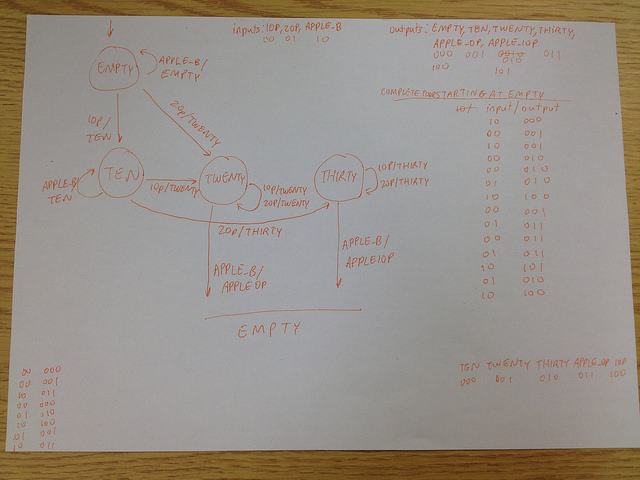
\includegraphics[width=350]{applefsm.jpg}
\caption{The manually created state machine for an Apple Vending Machine.}
\end{figure}
 
\begin{figure}
\centering
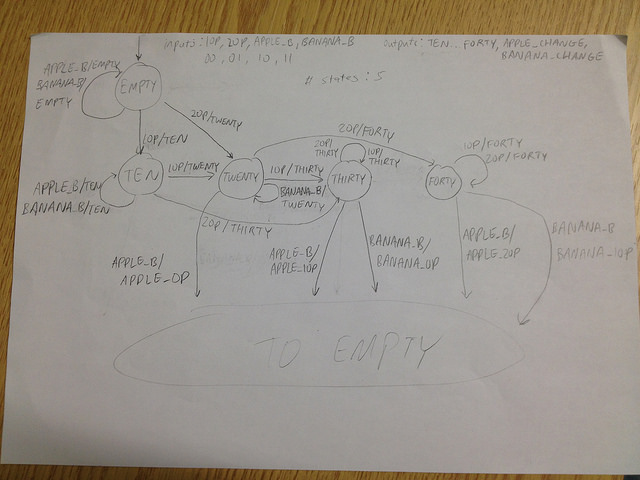
\includegraphics[width=350]{applebananafsm.jpg}
\caption{Manually created state machine for an Apple/Banana Vending Machine}
\end{figure}

\begin{figure}
\centering
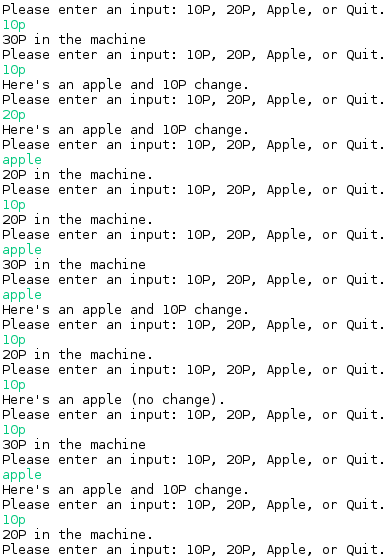
\includegraphics[width=350]{notworkingfsm.png}
\caption{The Apple vending machine not working correctly.}
\end{figure}

\begin{figure}
\centering
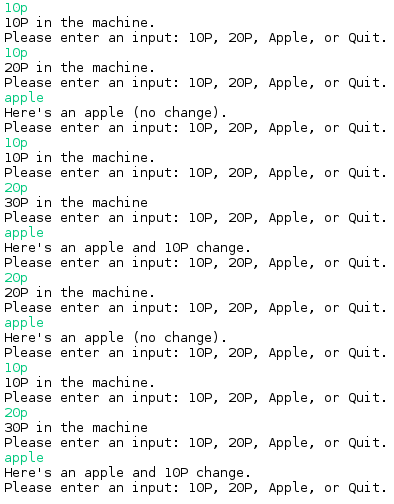
\includegraphics[width=350]{workingfsm.png}
\caption{The Apple vending machine working correctly.}
\end{figure}

\paragraph*{Documentation}
The self programming program is located in the selfprogramming directory. The jar for it is located in the jar directory.

Run the jar with
\begin{verbatim}
java -jar FSMLearning.jar
\end{verbatim}
Compile the code by running
\begin{verbatim}
make
\end{verbatim}
Run the code with
\begin{verbatim}
java -cp .:encog.jar AppleMachine 
\end{verbatim}

\begin{figure}
\centering
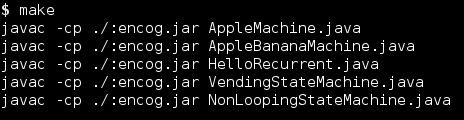
\includegraphics[width=350]{compileSL.png}
\caption{A screenshot of FSM compiling.}
\end{figure}
\begin{figure}
\centering
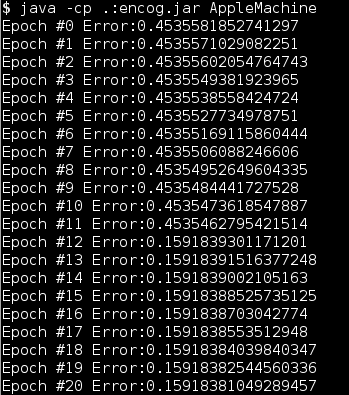
\includegraphics[width=350]{runSL.png}
\caption{A screenshot of FSM running.}
\end{figure}

\end{document}

